\subsection{A deblending test}
\label{sec:deblending_test}

In this section we demonstrate the performance of StarNet on deblending two stars. We simulated two stars in an $7\times 7$ image. 
We did not tile this image; the input to StarNet was the entire $7\times 7$ image.
We trained StarNet using the sleep phase, with prior described in Section~\ref{sec:gen_model}, except that we placed a uniform prior on the number of stars: with equal probability, there is either 0, 1, or 2 stars in the image. 

Figure~\ref{fig:deblending_test} displays the probability that $N = 2$ under our variational posterior, as the distance between two stars varies.
We also examine the effect of varying the fluxes and colors of stars. 
As the stars get brighter, the easier they become to deblend. As one star becomes brighter than the second star, the stars get harder to deblend. Finally, color differences between the stars aid in their deblending.
Across all the trials, the variational posterior reliably placed probability on two stars when the source separation is greater than one pixel. 

\begin{figure}[!h]
    \centering
    \begin{subfigure}{0.95\textwidth}
        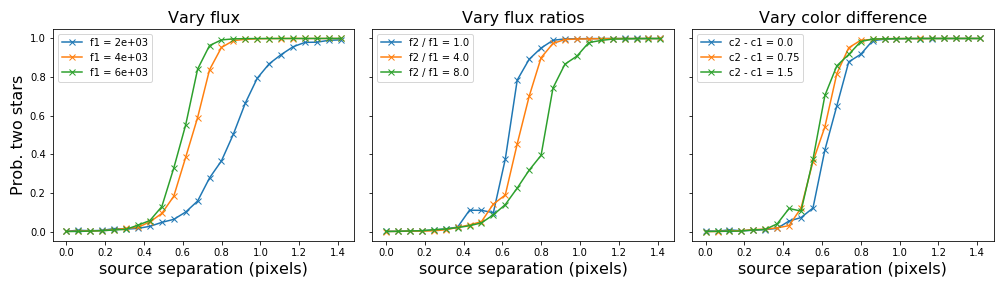
\includegraphics[width=\textwidth]{figures/deblending_test.png}
    \end{subfigure}
      \begin{subfigure}{0.95\textwidth}
        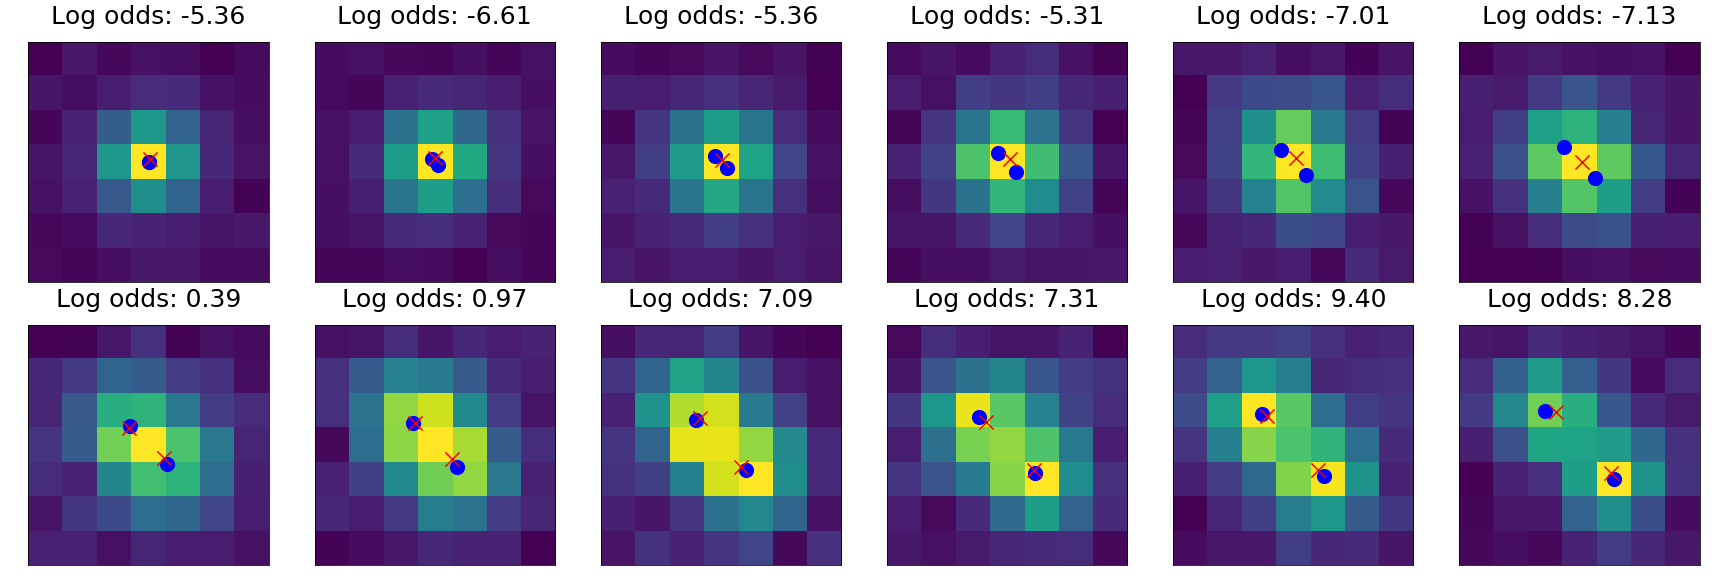
\includegraphics[width=\textwidth]{figures/deblending_ex_test.png}
    \end{subfigure}
    \label{eq:deblending_test}
    \caption{(Top) The probability under $q$ of two stars as source separation increases. On the left, both stars have the same flux, and their common flux was varied. In the middle, both stars have color = 0, and the first star had flux = 4000. We varied the flux of the second star to have the same, four times, or eight times the flux of the first star. On the right, both stars have $r$-band flux = 4000; the color of the first star is 0. The color of the second star was varied.
    (Bottom) An example of detections as source separation increases. Red are MAP detections, blue are true locations. Log odds are probability of two stars over probability of one star. Here, both stars have flux = 4000 and color = 0.}
    \label{fig:sparse_field}
\end{figure}
